
%!TEX program = xelatex
\documentclass[dvipsnames, svgnames,a4paper,11pt]{article}
% ----------------------------------------------------- 
%	加边框的命令
%	参考:https://tex.stackexchange.com/questions/531559/how-to-add-the-page-border-for-first-two-pages-in-latex
\usepackage{tikz}
\usetikzlibrary{calc}
\usepackage{eso-pic}
\AddToShipoutPictureBG{%
\begin{tikzpicture}[overlay,remember picture]
\draw[line width=0.6pt] % 边框粗细
    ($ (current page.north west) + (0.6cm,-0.6cm) $)
    rectangle
    ($ (current page.south east) + (-0.6cm,0.6cm) $); % 边框位置
\end{tikzpicture}}


\usepackage{xcolor}
\definecolor{c1}{HTML}{070F94} % 目录颜色 原版为2752C9 紫灰色535AAA 蓝紫色0B0DB7 深蓝色070F94 湖绿色219394 松石灰绿086173
\definecolor{c2}{HTML}{E20129} % 引用颜色 原版\definecolor{c2}{RGB}{190,20,83} 橙色F24729

\usepackage{ctex}
\usepackage[top=28mm,bottom=28mm,left=15mm,right=15mm]{geometry}
\usepackage{hyperref} 
\hypersetup{
	colorlinks,
	linktoc = section, % 超链接位置,选项有section, page, all
	linkcolor = c1, % linkcolor 目录颜色
	citecolor = c1  % citecolor 引用颜色
}
\usepackage{amsmath,enumerate,multirow,float}
\usepackage{tabularx}
\usepackage{tabu}
\usepackage{subfig}
\usepackage{fancyhdr}
\usepackage{graphicx}
\usepackage{wrapfig}  
\usepackage{physics}
\usepackage{appendix}
\usepackage{amsfonts}

%
\usepackage{tcolorbox}
\tcbuselibrary{skins,breakable}
\newtcolorbox{tbox}[2][]{
    colframe=black!70!,
    breakable,
    enhanced,
	boxrule =0.5pt,
    title = {#2},
    fonttitle = \large\kaishu\bfseries,
	drop fuzzy shadow,
    #1
}
\newtcolorbox[auto counter,number within=section]{question}[1][]{
  top=2pt,bottom=2pt,arc=1mm,
  boxrule=0.5pt,
%   frame hidden,
  breakable,
  enhanced, %跨页后不会显示下边框
  coltitle=c1!80!gray,
  colframe=c1,
  colback=c1!3!white,
  drop fuzzy shadow,
  title={思考题~\thetcbcounter:\quad},
  fonttitle=\bfseries,
  attach title to upper,
  #1
}

% ---------------------------------------------------------------------
%	利用cleveref改变引用格式,\cref是引用命令
\usepackage{cleveref}
\crefformat{figure}{#2{\textcolor{c2}{Figure #1}}#3} % 图片的引用格式
\crefformat{equation}{#2{(\textcolor{c2}{#1})}#3} % 公式的引用格式
\crefformat{table}{#2{\textcolor{c2}{Table #1}}#3} % 表格的引用格式


% ---------------------------------------------------------------------
%	页眉页脚设置
\fancypagestyle{plain}{\pagestyle{fancy}}
\pagestyle{fancy}
\lhead{\kaishu 中山大学物理与天文学院基础物理实验\uppercase\expandafter{\romannumeral2}} % 左边页眉,学院 + 课程
\rhead{\kaishu 实验报告By黄罗琳} % 右边页眉,实验报告标题
\cfoot{\thepage} % 页脚,中间添加页码


% ---------------------------------------------------------------------
%	对目录、章节标题的设置
\renewcommand{\contentsname}{\centerline{\huge 目录}}
\usepackage{titlesec}
\usepackage{titletoc}
% \titleformat{章节}[形状]{格式}{标题序号}{序号与标题间距}{标题前命令}[标题后命令]
\titleformat{\section}{\centering\LARGE\songti}{}{1em}{}

% ---------------------------------------------------------------------
%   listing代码环境设置
\usepackage{listings}
\lstloadlanguages{python}
\lstdefinestyle{pythonstyle}{
backgroundcolor=\color{gray!5},
language=python,
frameround=tftt,
frame=shadowbox, 
keepspaces=true,
breaklines,
columns=spaceflexible,                   
basicstyle=\ttfamily\small, % 基本文本设置,字体为teletype,大小为scriptsize
keywordstyle=[1]\color{c1}\bfseries, 
keywordstyle=[2]\color{Red!70!black},   
stringstyle=\color{Purple},       
showstringspaces=false,
commentstyle=\ttfamily\scriptsize\color{green!40!black},%注释文本设置,字体为sf,大小为smaller
tabsize=2,
morekeywords={as},
morekeywords=[2]{np, plt, sp},
numbers=left, % 代码行数
numberstyle=\it\tiny\color{gray}, % 代码行数的数字字体设置
stepnumber=1,
rulesepcolor=\color{gray!30!white}
}




% ---------------------------------------------------------------------
%	其他设置
\def\degree{${}^{\circ}$} % 角度
\graphicspath{{./images/}} % 插入图片的相对路径
\allowdisplaybreaks[4]  %允许公式跨页 
\usepackage{lipsum}
\usepackage{adjustbox}
%\usepackage{mathrsfs} % 字体
%\captionsetup[figure]{name=Figure} % 图片形式
%\captionsetup[table]{name=Table} % 表格形式

\begin{document}
	
	
	
	% 实验报告封面	
	
	% 顶栏
	\begin{table}
		\renewcommand\arraystretch{1.7}
		\begin{tabularx}{\textwidth}{
				|X|X|X|X
				|X|X|X|X|}
			\hline
			\multicolumn{2}{|c|}{预习报告}&\multicolumn{2}{|c|}{实验记录}&\multicolumn{2}{|c|}{分析讨论}&\multicolumn{2}{|c|}{总成绩}\\
			\hline
			\LARGE25 & & \LARGE 30& & \LARGE25 & & \LARGE80 & \\
			\hline
		\end{tabularx}
	\end{table}
	% ---
	
	
	\begin{table}
		\renewcommand\arraystretch{1.7}
		\begin{tabularx}{\textwidth}{|X|X|X|X|}
			\hline
			专业: &  物理学 &年级: & 2022级\\
			\hline
			姓名: & 黄罗琳 & 学号: & 22344001\\
			\hline
			实验时间: & 2024.3.7 & 教师签名:见后 & \\
			\hline
		\end{tabularx}
	\end{table}
	% ---
	
	% 大标题
	\begin{center}
		\LARGE 实验 CC3 \quad 双光栅测量微弱振动位移量实验
	\end{center}
	% ---
	
	% 注意事项
	
	% 基本
	\textbf{【实验报告注意事项】}
	\begin{enumerate}
		\item 实验报告由三部分组成:
		\begin{enumerate}
			\item 预习报告:课前认真研读实验讲义,弄清实验原理;实验所需的仪器设备、用具及其使用、完成课前预习思考题;了解实验需要测量的物理量,并根据要求提前准备实验记录表格(可以参考实验报告模板,可以打印)。\textcolor{red}{\textbf{(20分)}}
			\item 实验记录:认真、客观记录实验条件、实验过程中的现象以及数据。实验记录请用珠笔或者钢笔书写并签名(\textcolor{red}{\textbf{用铅笔记录的被认为无效}})。\textcolor{red}{\textbf{保持原始记录,包括写错删除部分,如因误记需要修改记录,必须按规范修改。}}(不得输入电脑打印,但可扫描手记后打印扫描件);离开前请实验教师检查记录并签名。\textcolor{red}{\textbf{(30分)}}
			\item 数据处理及分析讨论:处理实验原始数据(学习仪器使用类型的实验除外),对数据的可靠性和合理性进行分析;按规范呈现数据和结果(图、表),包括数据、图表按顺序编号及其引用;分析物理现象(含回答实验思考题,写出问题思考过程,必要时按规范引用数据);最后得出结论。\textcolor{red}{\textbf{(30分)}}
		\end{enumerate}
		\textbf{实验报告就是将预习报告、实验记录、和数据处理与分析合起来,加上本页封面。\textcolor{red}{(80分)}}
		\item 实验报告就是将预习报告、实验记录、分析讨论合起来,加上本页封面。实验记录须手写,预习报告和分析讨论部分手写或打印均可。
		\item 每次完成实验后的一周内交实验报告(特殊情况不能超过两周),每份报告必须注明姓名和学号,合作者和学号,否则按零分处理。 
		\item \textbf{安全注意事项}:
		\begin{enumerate}
			\item 实验过程中,光源不要随意打开关闭;
			\item 严禁用手触光学镜头的表面;
			\item 严禁用强力和斜向力旋转测微头,这样会损坏测微头或其他部件;
			\item 不要拆卸传动机构,以免影响仪器正常使用;
			\item 实验过程中,数条纹时,避免桌面的振动。
			
		\end{enumerate}
	\end{enumerate}
	

	
	
	% 目录
	\clearpage
	\tableofcontents
	\clearpage
	% ---
	
	
	
	% 预习报告	
	
	% 小标题
	\setcounter{section}{0}
	\section{双光栅测量微弱振动位移量实验 \quad\heiti 预习报告}
	% ---
	
	% 实验目的
	\subsection{实验目的}
	\begin{enumerate}
		\item 了解利用光的多普勒频移形成光拍的原理并用于测量光拍拍频。
		\item 学会使用精确测量微弱振动位移的一种方法。
		\item 应用双光栅微弱振动测量仪测量音叉振动的微振幅
	\end{enumerate}
	% ---
	
	% 仪器用具
	\subsection{仪器用具}
	\begin{table}[htbp]
		\centering
		\renewcommand\arraystretch{1.6}
		% \setlength{\tabcolsep}{10mm}
		\begin{tabular}{p{0.05\textwidth}|p{0.20\textwidth}|p{0.05\textwidth}|p{0.5\textwidth}}
		
			\hline
			编号& 仪器用具名称 & 数量 &  主要参数(型号,测量范围,测量精度等) \\
			\hline
			1& 双光栅微弱振动测量仪 & 1 & DHGS-1 型,半导体激光器: λ=650nm,功
			率 2-5mW;音叉谐振频率: 500Hz 左右。\\
			
				2&数字示波器& 1 &  DS1000E(D)\\
			
				3& 信号发生器 & 1 &  MFG-2000\\
		
				
			\hline
		
		\end{tabular}
	\end{table}
	% ---
	
	% 原理概述
	\subsection{实验原理}
	\begin{enumerate}
		\item 位移光栅的多普勒频移\\
		因多普勒效应产生的频率变化称为多普勒频移。 图1的位相光栅与振幅光栅(由透光部分和不透光部分组成)不同,它是利用不同的光密和光疏媒质部分对同一束单色光产生的光程差的不同而导致入射的平面波发生畸变。
		\begin{figure}[H]
			\centering
			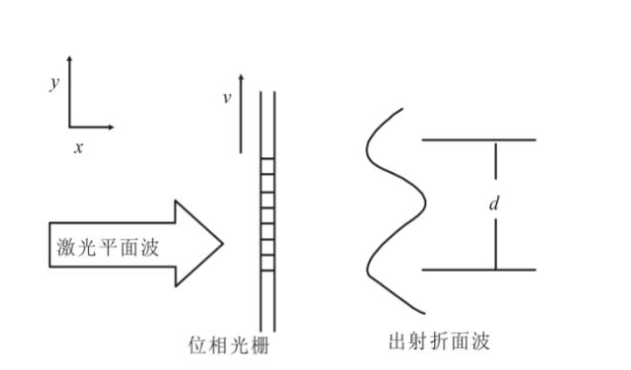
\includegraphics[width=0.5\linewidth]{images/出射的折曲面波阵面}
			\caption{出射的折曲面波阵面}
			\label{fig:出射的折曲面波阵面}
		\end{figure}
		现推导位移光栅的多普勒频移公式。\\
		激光平面波入射到光栅,由于光栅上缝自身和每缝之间的衍射作用,通过光栅后光的强度出现周期性的变化。远场可得:$a(sin\theta_m-sin\theta_i)=m\lambda,\quad m\in N$
		其中,$a$是光栅常数;$\theta_m$第 m 级谱线对应的折射角;$\theta_i$是入射角(本实验中$\theta_i=0$),$\lambda$为波长。
		如果光栅在 y 方向以速度 v 移动, 由于可以理解为积分原点以速度 v 移动,则从光栅出射的光的波阵面也以速度 v 在 y 方向移动。 因此在不同时刻,对应于同一级的衍射光射,它从光栅出射时,在 y 方向也有一个 𝑣𝑡 的位移量。
		\begin{figure}[H]
			\centering
			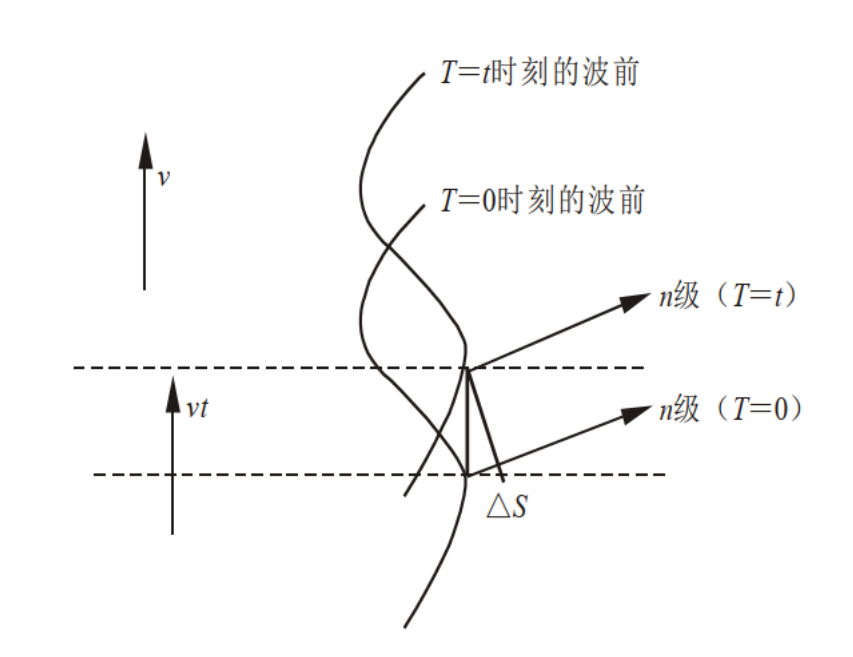
\includegraphics[width=0.5\linewidth]{images/衍射光线位移量}
			\caption{衍射光线位移}
			\label{衍射光线位移}
		\end{figure}
		这个位移量对应于出射光波位相的变化量为 $\Delta\varphi(t)$
		
		$$\Delta\varphi(\mathfrak{t})=\mathrm{k}_0\Delta\mathfrak{s}=\mathrm{k}_0\nu tsin\theta $$ \\
		最终可得:
		$\Delta\varphi(\mathfrak{t})=2\pi\mathrm{m}\frac vdt=\mathrm{m}\omega_dt$
		此为就是移动的位相光栅 m 级衍射光波与静止的位相光栅衍射光波的相位差。
		\begin{figure}[H]
			\centering
			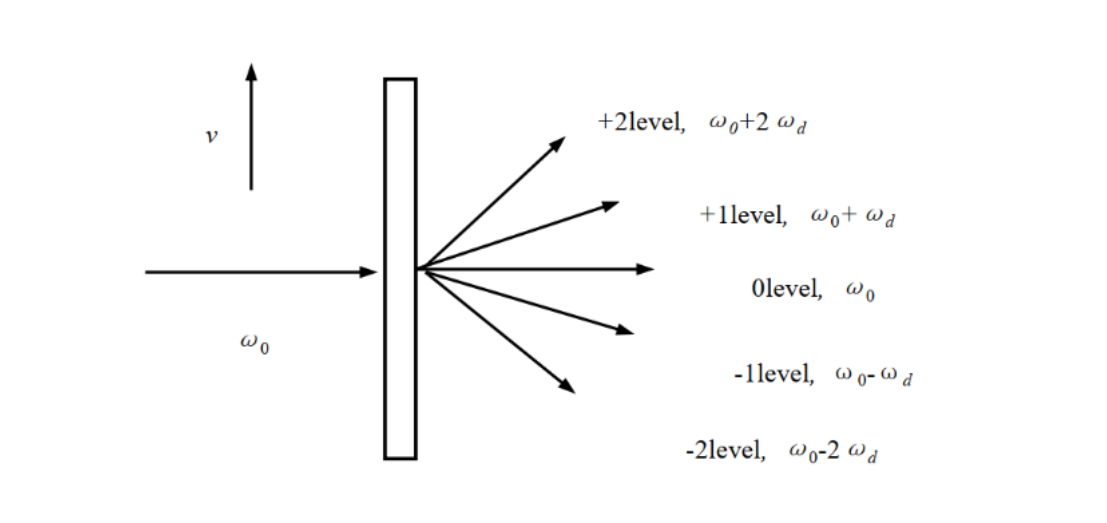
\includegraphics[width=0.5\linewidth]{images/移动光栅的多普勒频移}
			\caption{移动光栅的多普勒频移}
			\label{移动光栅的多普勒频移}
		\end{figure}
		
		
		\item 2. 光拍的获得与检测 \\
		光频率很高,为了在光频$^{\omega_0}$中检测出多普勒频移量,必须采用“拍”的方法,即要把已频移的和未频移的光束互相平行迭加,以形成光拍。由于拍频较低,容易测得,通过拍频即可检测出多普勒频移量。
		
		本实验形成光拍的方法是采用两片完全相同的光栅平行紧贴,一片 B 静止,另一片 A 相对移动。激光通过双光栅后所形成的衍射光,即为两种以上光束的平行迭加。由于双光栅紧贴,激光束具有一定宽度,故该光束能平行迭加,这样直接而又简单地形成了光拍。\\
		将$I=\xi(E_1+E_2)^2$展开后舍去无法检测项。
		
		$$i_s=\zeta E_{10}E_{20}\cos\left[\omega_dt+(\omega_2-\omega_1)\right]$$ \\
		拍频即为:
		$$
		F=\frac{\omega_d}{2\pi}=\frac{\nu_A}d=\nu_An_\theta 
		$$
		
		其中,$n_\theta$是光栅密度,本实验中$n_\theta=100mm^{-1}$。
		
	\item 微弱振动位移量的检测\\
		从式(5)可知,由于$n_\mathrm{\theta}$是常数且$\upsilon_\mathrm{A}$随时间周期变化,故微弱振动的位移振幅为:
		
		$$
		A=\frac12\int_0^{\Large\frac T2}\nu(t)dt=\frac1{2n_\theta}\int_0^{\Large\frac T2}F(t)dt\quad(6)
		$$
		
		其中,$\int_0^{T/2}F(t)dt$表示在T/2 时间内的拍频波的个数,所以只要测得拍频波的波数, 就可得到较弱振动的位移振幅。
		
		波形数由完整波形数、波的首数、波的尾数三部分组成。波形数n为:
		$n=n_0+\frac12$
		其中,$n_0$为完整波形数,a、b 为波群的首、尾幅度和该处完整波形的振幅之比,
		$sin^{-1}a$和$sin^{-1}b$的取值范围是0~360°, 所以要注意不完整波形中是否出现波峰和波谷。例如,在下图中,由于首波恰好完整,而尾部出现了一个波峰,故:
		
		$$
		n=n_0+\frac{sin^{-1}b}{360°}=4+\frac{113.6°}{360°}=4.32
		$$
		
	\end{enumerate}
	% ---
	
	`
	
	% 实验前思考题
	\subsection{预习思考题}
	请见实验原理部分

	
	
	
	
	% 实验记录	
	\clearpage
	
	% 顶栏
	\begin{table}
		\renewcommand\arraystretch{1.7}
		\centering
		\begin{tabularx}{\textwidth}{|X|X|X|X|}
			\hline
			专业: & 物理学 & 年级: & 2022级 \\
			\hline
			姓名: & 黄罗琳 & 学号: & 22344001\\
			\hline
			室温: &  25℃& 实验地点: & A511 \\
			\hline
			学生签名: & 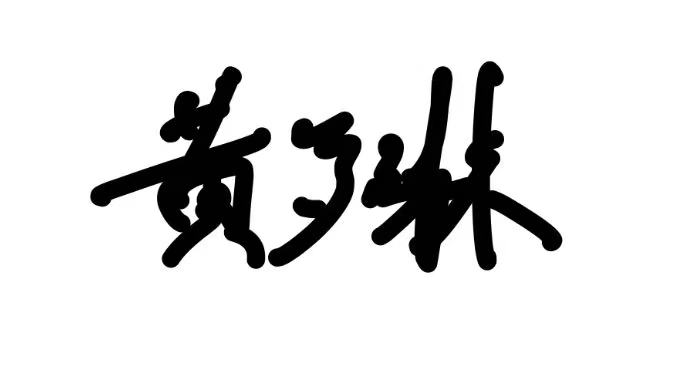
\includegraphics[width=1cm]{签字.jpg} &
    评分: & \\
			\hline
			实验时间:& 2024/3/7 & 教师签名:&\\
			\hline
		\end{tabularx}
	\end{table}
	% ---
	
	% 小标题
	\section{双光栅测量微弱振动位移量实验 \quad\heiti 实验记录}
	% ---
	
	% 实验过程记录
	\subsection{实验内容、步骤与结果}
	
	%
	\subsubsection{实验完整步骤简述}
	\begin{enumerate}
		\item 将固纬信号发生器的 CH1 通道连接至光学实验平台音叉驱动器(动光栅),输出频率约为 500 Hz、Vpp 约为 6 V 的正弦波驱动信号。
		
		\item 将光学实验平台光电传感器输出信号连接至示波器的 CH1 通道。因为光电传感器输出信号功率较低,示波器 CH1 探头选择放大约 500 倍。
		
		\item 将固纬信号发生器同步信号输出,连接至示波器 CH2 作为触发源。

		
		\item 光路调整:将激光器接至半导体激光电源,静光栅、动光栅排成一直线。调节静光栅和动光栅位置,使其平行。调整至形成竖排衍射光斑,调节至中间最亮光斑进入光电传感器。
		
		\item 音叉谐振调节:调整音叉和激振换能器间距至约 0.3mm。将固纬信号发生器 CH1 通道连接至光学实验平台音叉驱动器(动光栅),输出频率约为 500 Hz、Vpp 约为 6 V 的正弦波驱动信号。微调频率至音叉谐振(振幅最大)。调节时,轻触音叉顶部感受振动强度或听振动声音。若振动太强,减小驱动信号幅度。示波器上波数约为 15 个。记录此时音叉振动频率、完整波数、不足一个完整波形的首尾数值以及对应振幅值。
		
		\item 测量外力驱动音叉时的谐振曲线。在音叉谐振点附近,调节驱动信号频率,测量振动频率与振幅大小,频率间隔为 0.1 Hz,选取 8 个点。保持驱动信号幅度不变,通过调节音叉上小孔中软管,改变音叉的有效质量,观察谐振曲线的变化趋势。
	\end{enumerate}
	\begin{figure}[H]
		\centering
		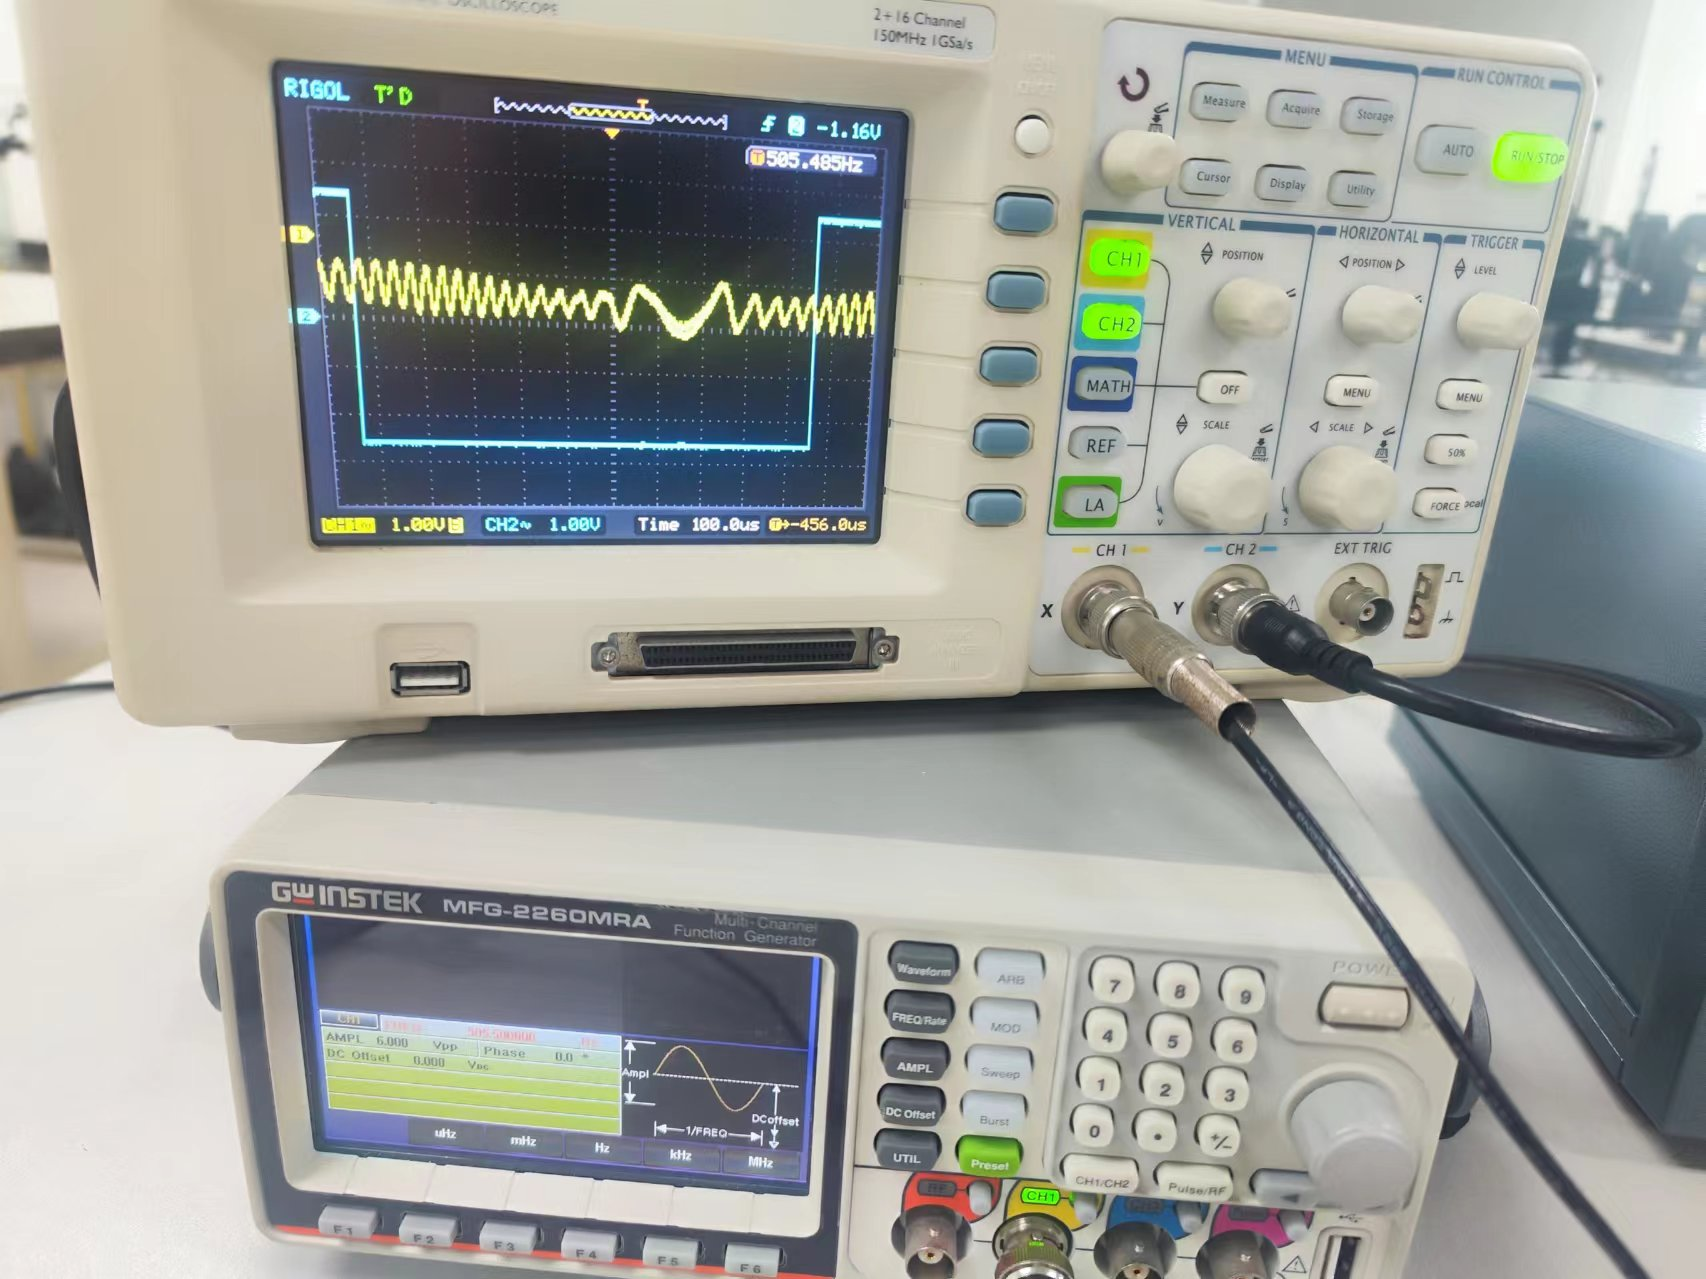
\includegraphics[width=0.4\linewidth]{images/实验剪影1}
		\caption{未插入软管实验效果示例}
		\label{实验剪影1}
	\end{figure}
	\begin{figure}[H]
		\centering
		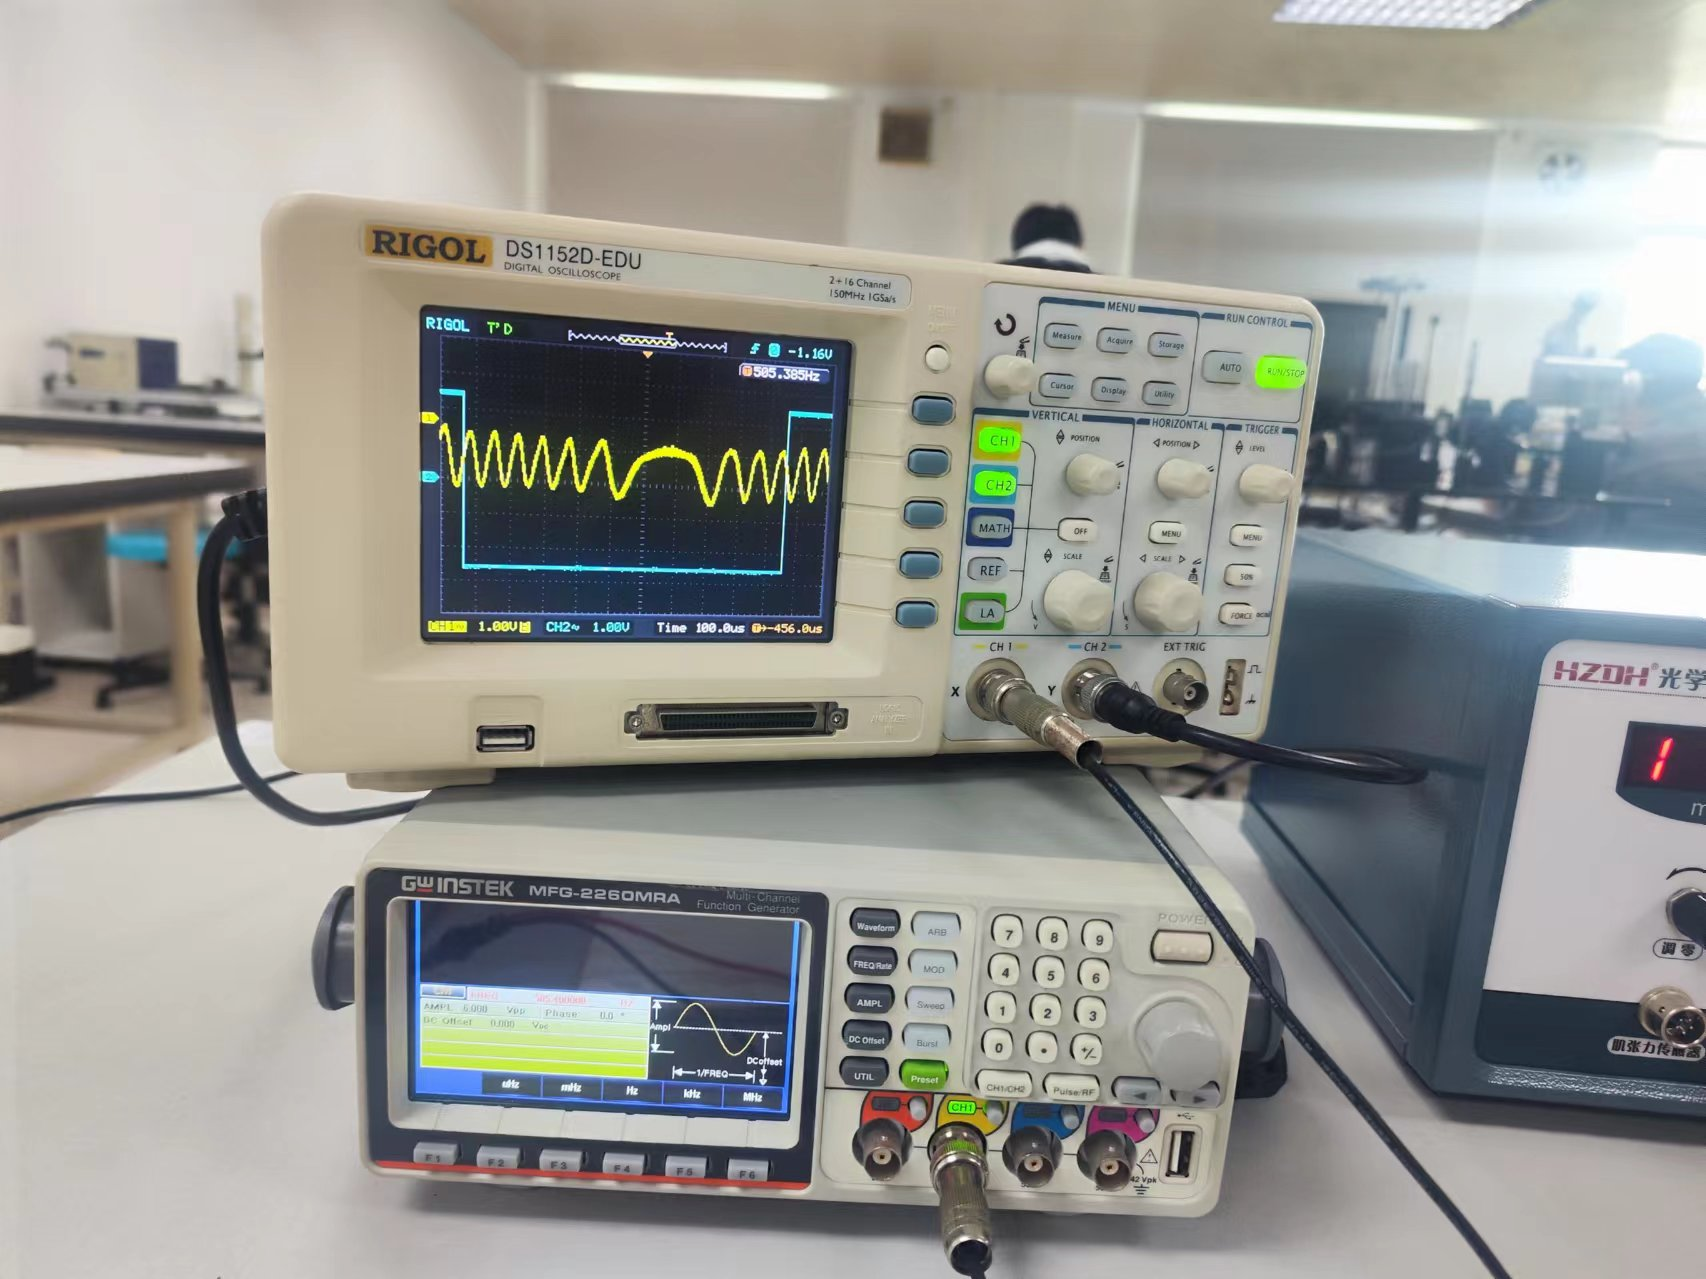
\includegraphics[width=0.4\linewidth]{images/实验剪影2}
		\caption{插入软管后实验效果示例}
		\label{实验剪影2}
	\end{figure}
	\begin{figure}[H]
		\centering
		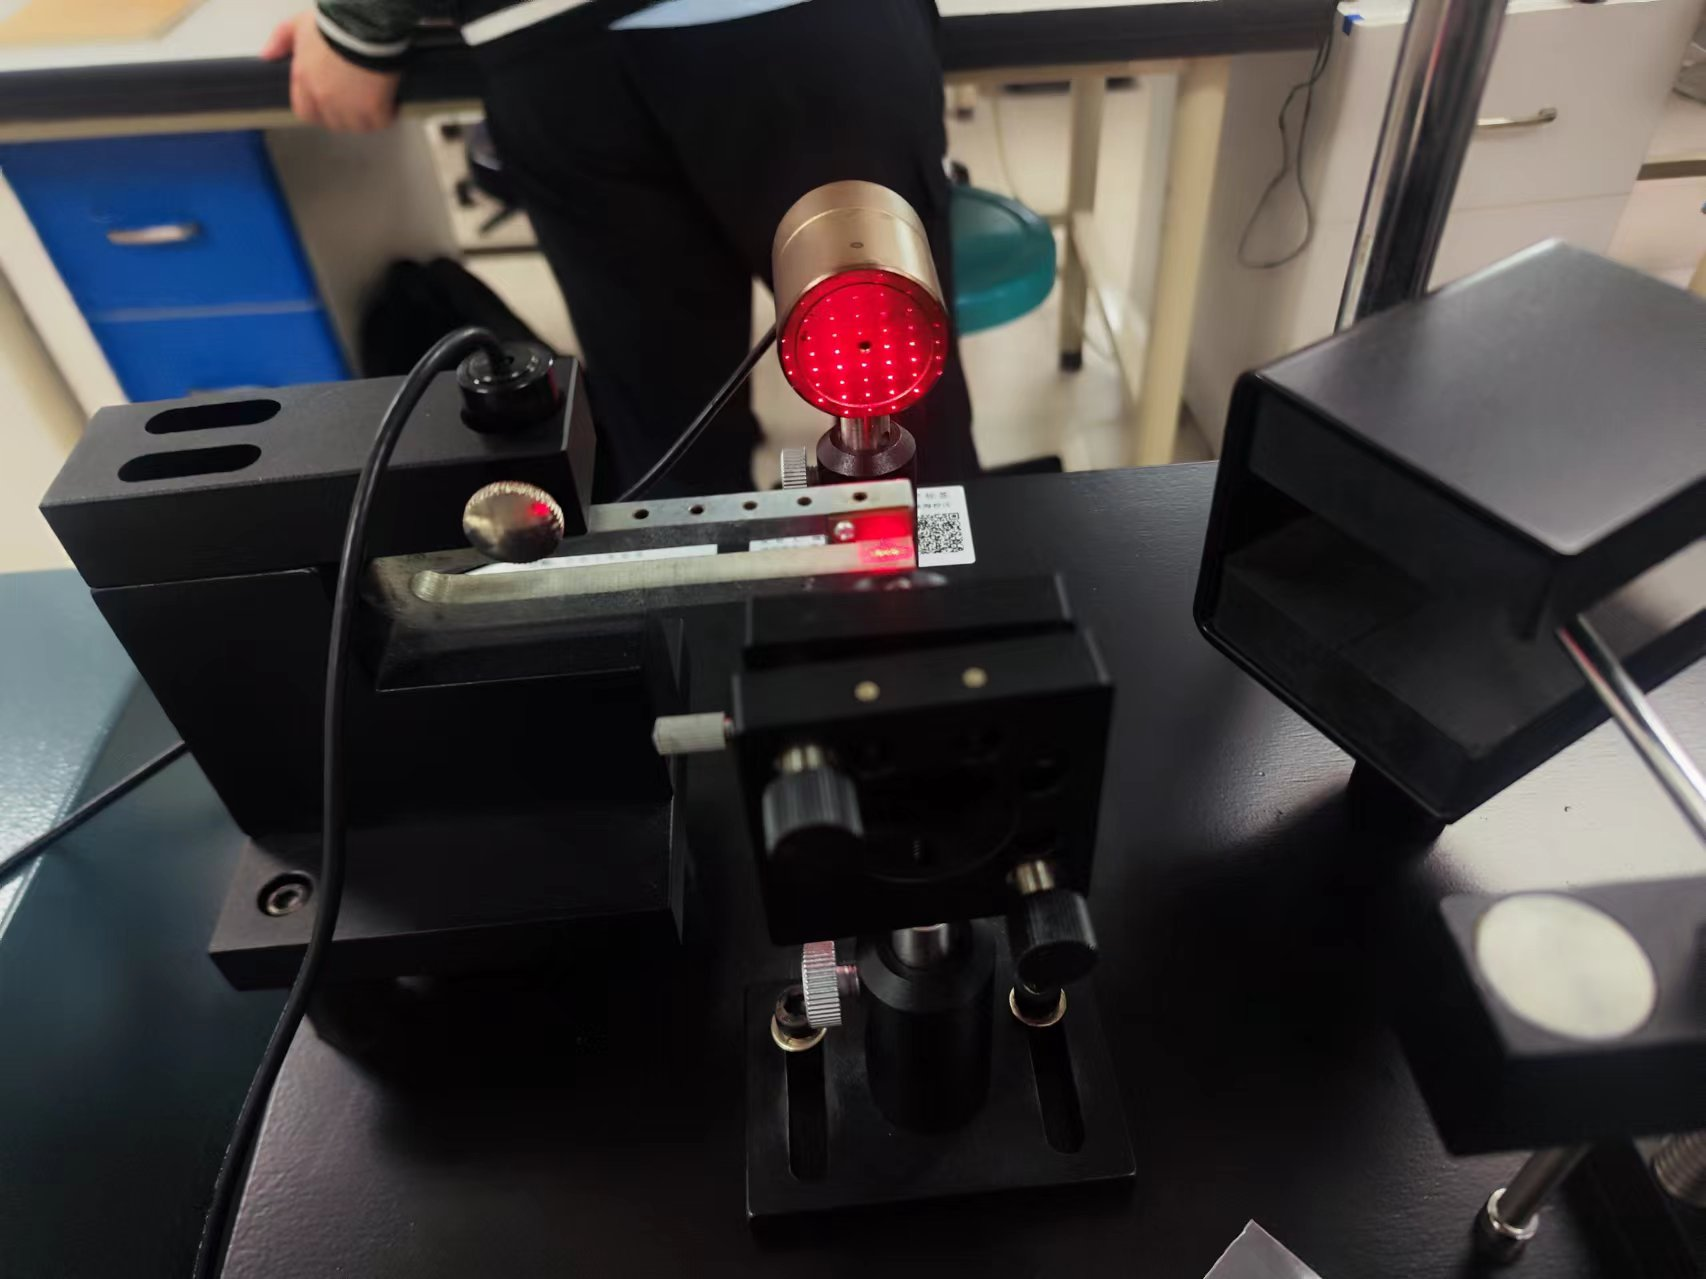
\includegraphics[width=0.4\linewidth]{images/错误}
		\caption{实验中错误光路}
		\label{}
	\end{figure}
	注:实验效果相对较好,难点在于调整光路和仪器,得到正确的实验图像后,相关内容比较简单。
		\subsubsection{实验数据整理}
		\begin{table}[H]
			\centering
			\begin{tabular}{|l|l|l|}
			\hline
			频率/HZ & 波数    & 振幅      \\ \hline
			505.3 & 6.45  & 0.03225 \\ \hline
			505.4 & 9.45  & 0.04725 \\ \hline
			505.5 & 21.25 & 0.10625 \\ \hline
			\textbf{505.6} & \textbf{37.54} & \textbf{0.1877}  \\ \hline
			505.7 & 18.54 & 0.0927  \\ \hline
			505.8 & 10.52 & 0.0526  \\ \hline
			505.9 & 7.57  & 0.03785 \\ \hline
			506   & 5.45  & 0.02725 \\ \hline
			506.1 & 4.36  & 0.0218  \\ \hline
			506.2 & 3.55  & 0.01775 \\ \hline
			506.3 & 3.25  & 0.01625 \\ \hline
			506.4 & 2.53  & 0.01265 \\ \hline
			506.5 & 2.45  & 0.01225 \\ \hline
			506.6 & 2.4   & 0.012   \\ \hline
			\end{tabular}
			\caption{未加软管前实验数据(谐振点加粗)}
			\label{未加软管前实验数据}
		\end{table}
		
		\begin{table}[H]
			\centering
			\begin{tabular}{|l|l|l|}
			\hline
			频率/HZ & 波数    & 振幅      \\ \hline
			504.5 & 3.26  & 0.0163 \\ \hline
			504.6 & 4.4   & 0.022  \\ \hline
			504.7 & 5.46  & 0.0273 \\ \hline
			504.8 & 8.28  & 0.0414 \\ \hline
			504.9 & 11.9  & 0.0595 \\ \hline
			\textbf{505} & \textbf{19.15} & \textbf{0.09575} \\ \hline
			505.1 & 13.5  & 0.0675 \\ \hline
			505.2 & 8.65  & 0.04325 \\ \hline
			505.3 & 7.53  & 0.03765 \\ \hline
			\end{tabular}
			\caption{加软管后实验数据(谐振点加粗)}
			\label{加软管后实验数据}
		\end{table}
	
		
	
	
	

	% 问题记录
	\subsection{实验过程遇到问题及解决办法}
	\begin{enumerate}
		\item 在实验过程中,起初并没有得到合适的信号图像,通过调整焦距,距离,以及可能会存在光线打到音叉上等一些操作问题,导致我用了好长时间来对实验仪器进行调整,最终得到了初步可用的实验图像,从而继续实验。
		\item 实验有一些仪器存在问题,例如激光亮度不够,仪器接收不到信号,此现象为某一台仪器上只存在CH2的方波(蓝色)显示,而CH1对应的黄线根本不会随着光路的调整而产生变化,初步认定为是光电传感器的问题。
		\item 此外在实验过程中可以明显感觉出实验受到外界影响严重,其中一点桌子的微弱震动都会影响到曲线的形成,从而影响计数。
		\item 对于计数问题,实验原有的计数方法仅仅适用于波数较少的情况,若屏幕上显示波数较多,则只能初步估算出波数,但是根据实验来看,只有谐振点附近的波数会比较多,其余情况还是可以利用计算得出具体的波数。
	\end{enumerate}

	
	
	% 分析与讨论	
	\clearpage
	
	% 顶栏
	\begin{table}
		\renewcommand\arraystretch{1.7}
		\begin{tabularx}{\textwidth}{|X|X|X|X|}
			\hline
			专业:& 物理学 &年级:& 2022级\\
			\hline
			姓名: & 黄罗琳 & 学号:& 22344001\\
			\hline
			日期:& 2024/3/14 & 评分: &\\
			\hline
		\end{tabularx}
	\end{table}
	% ---
	
	% 小标题
	\section{双光栅测量微弱振动位移量实验 \quad\heiti  分析与讨论}
	% ---
	
	% 数据处理
	\subsection{实验数据分析}
	
	\subsubsection{音叉谐振时光拍信号的平均频率}
	\begin{enumerate}
		\item 实验结果计算\\
		根据实验测量数据得知,音叉谐振频率为:505.6HZ\\
		波数:37.54\\
	    根据平均频率计算公式可得:
	  $$\tilde{F}=\frac{2}{T}\int_{0}^{\frac{T}{2}}F(t)dt=2\times505.6\times37.54=37960.488\text{hz}$$
	  \item 实验结果分析\\
	  从实验结果来看,似乎频率非常高,初步分析可能是由于在测量过程中由于示波器读数的问题,从下图可知,当时示波器显示的波数相当密集,对照所有实验操作步骤很数据总体趋势来看,似乎并无差错,可能由于实验仪器的缘故,导致数值偏大。

	  \begin{figure}[H]
		\centering
		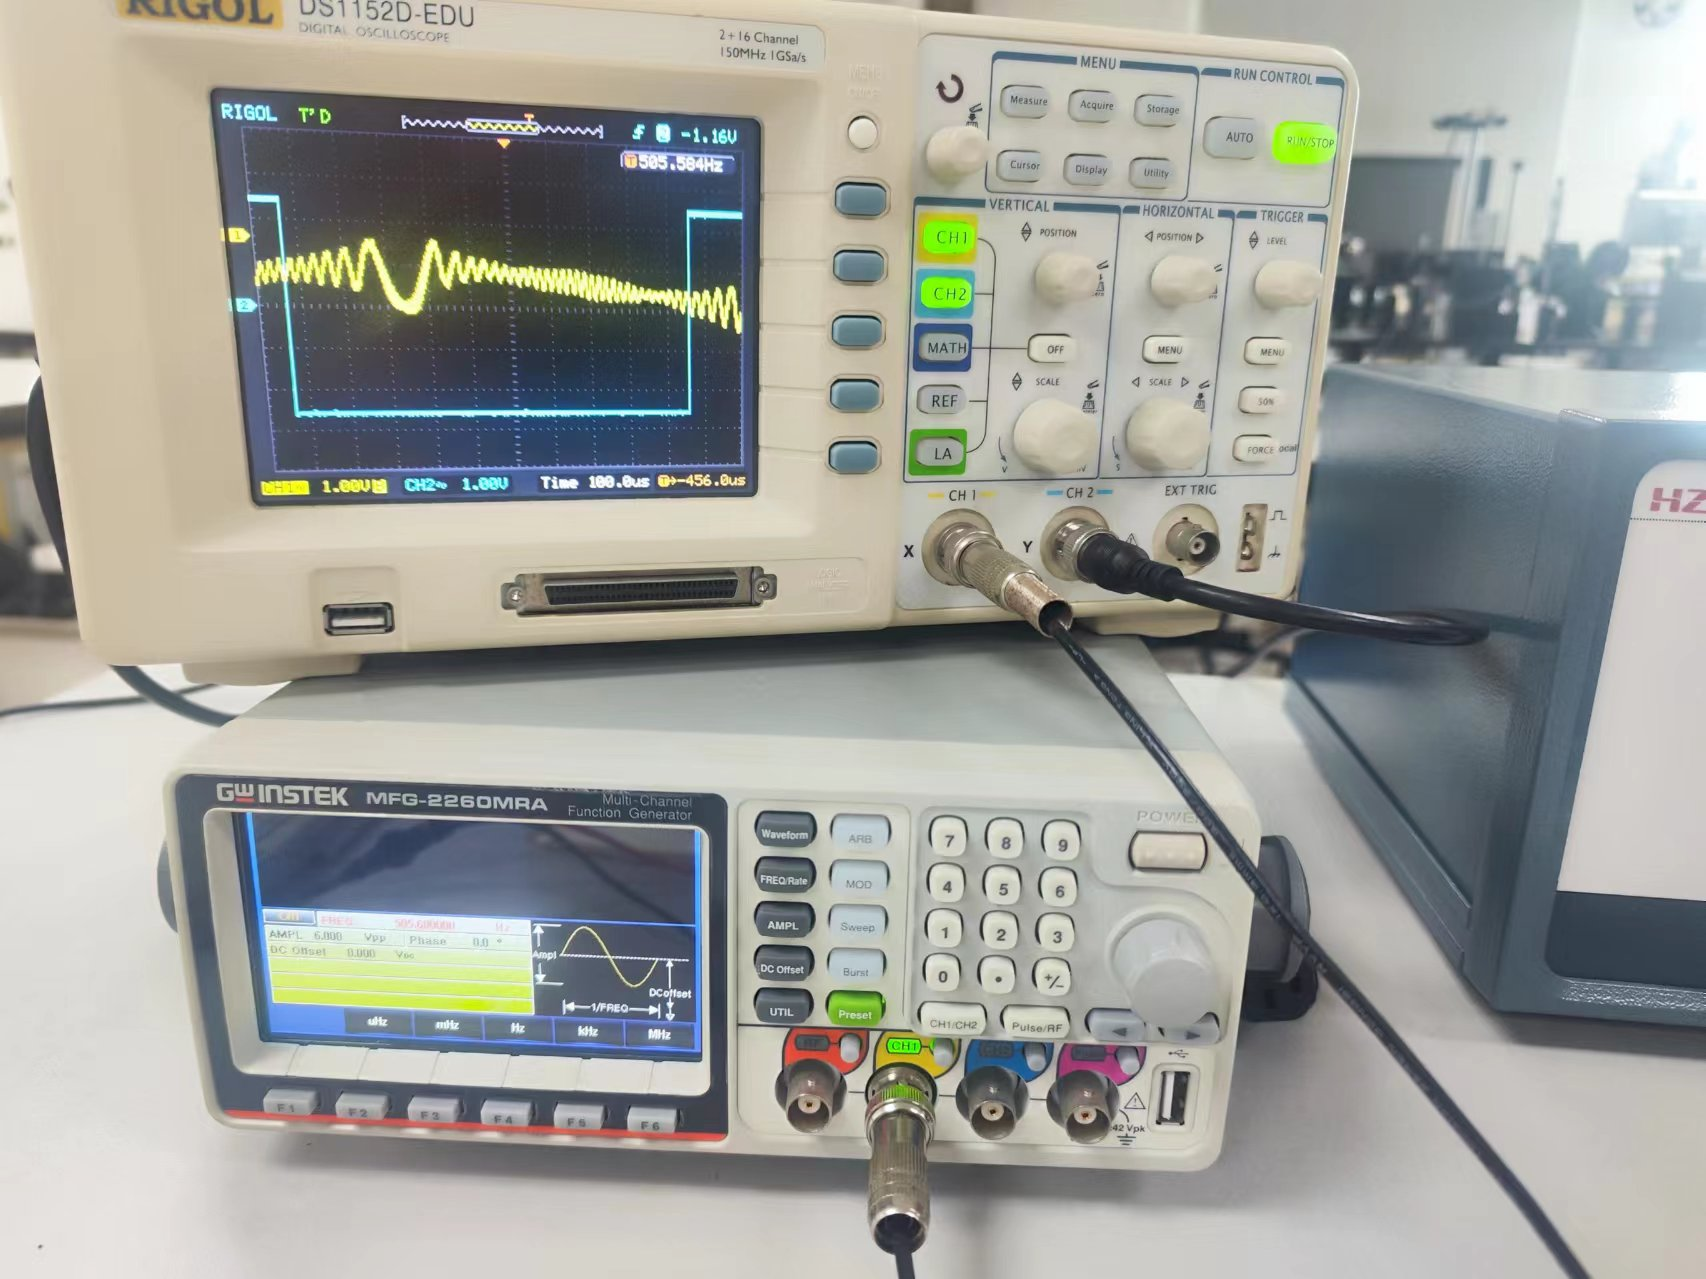
\includegraphics[width=0.4\linewidth]{images/505.6}
		\caption{谐振频率(505.6HZ)实验图像}
		\label{505.6}
	\end{figure}
	  
	\end{enumerate}
	
	%
	\subsubsection{ 音叉在谐振点时作微弱振动的位移振幅}
	$$\begin{aligned}A=\frac{1}{2n_\theta}\int_0^{\frac{T}{2}}F(t)dt=0.1877\text{mm}\end{aligned}$$
	\subsection{实验数据讨论}
	\subsubsection{ 画出音叉的频率—振幅曲线;分析讨论其特点}
	如图所示,使用Origin软件进行图形绘制。
	\begin{figure}[H]
		\centering
		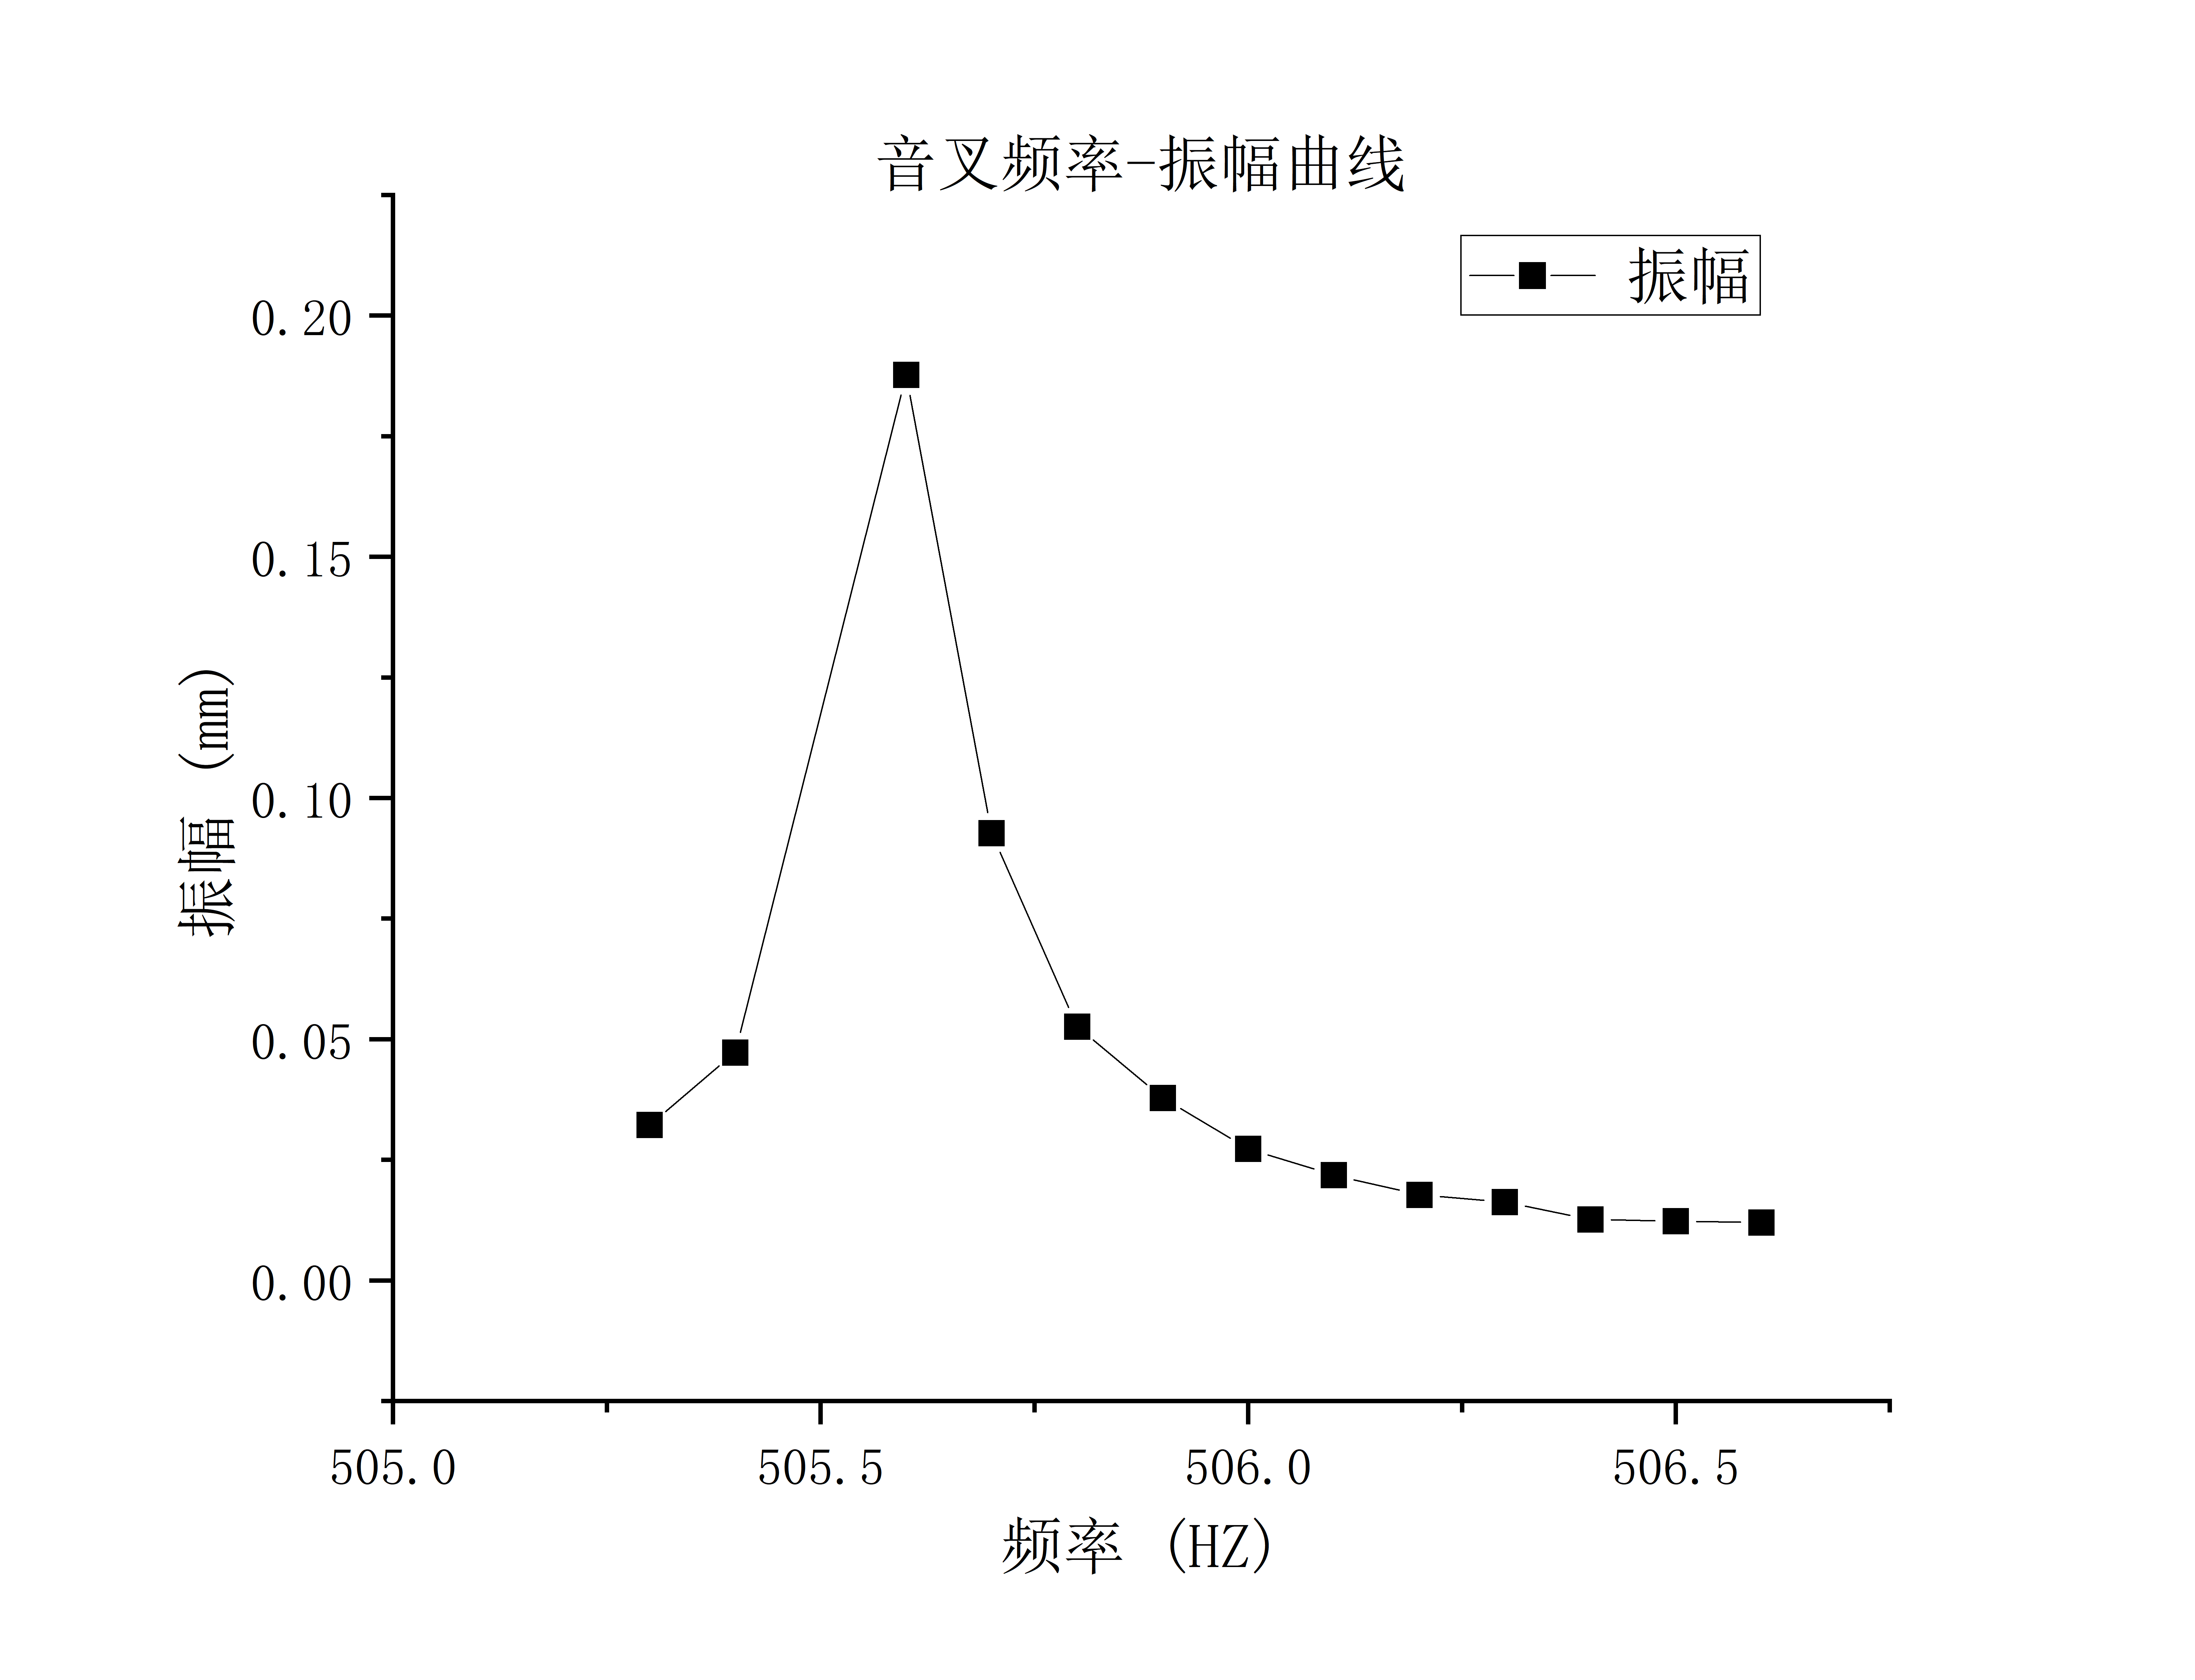
\includegraphics[width=0.8\linewidth]{images/振幅曲线}
		\caption{频率—振幅曲线}
		\label{频率—振幅曲线}
	\end{figure}
	初步分析图像可得如下结论:
	\begin{enumerate}
		\item \textbf{尖峰图像:} 此图像的形状是一个尖峰,这说明了在谐振频率附近,振幅会达到最大值。这是因为在谐振频率处,音叉受到的外部驱动与其固有频率完全匹配,导致振幅增加到最大。
		
		\item \textbf{振幅对频率的敏感性:} 振幅对频率的改变比较敏感。这意味着在谐振频率附近,即使微小的频率变化也会导致振幅发生显著的变化。这是因为在谐振频率附近,小的频率变化会导致外部驱动与固有频率的匹配程度发生变化,进而影响振幅的大小。
		
		\item \textbf{图像斜率的绝对值较大:} 在谐振频率附近,图像的斜率绝对值较大。在图像中,斜率代表了振幅随频率变化的速率。较大的斜率意味着在谐振频率附近,即使微小的频率变化也会导致振幅发生较大的变化。
		
		\item \textbf{距离谐振频率越远,曲线的斜率越小:} 在远离谐振频率处,曲线的斜率越小。这意味着当远离谐振频率时,外部驱动的频率变化不会显著影响振幅,因为音叉不再处于与驱动频率相匹配的状态,振幅的变化程度较小。
	\end{enumerate}
	\subsubsection{作出音叉不同有效质量时的谐振曲线,分析讨论其变化趋势}
	
	
	\textbf{分析图实验中通过在音叉的圆孔处插入软管,从而做到了改变音叉的有效质量,进一步改变其谐振频率,具体趋势如图9所示:并且与图8进行比较,可以得出:}
	
	\begin{enumerate}
		\item \textbf{不同质量下的幅频曲线}:
		\begin{itemize}
			\item 幅频曲线具有相同的特征,即存在一个明显的尖峰,对应着谐振频率的位置。
			\item 在谐振频率附近,曲线的斜率绝对值很大,表明振幅对频率的变化非常敏感。随着频率偏离谐振频率,曲线的斜率逐渐减小。
		\end{itemize}
		\item \textbf{加软管后的实验数据对比}:
		\begin{itemize}
			\item 实验结果显示,加上软管后,音叉的谐振频率减小了。
			\item 根据公式 $\omega=\sqrt{\frac{k}{m}}$,质量增加会导致谐振频率减小。
		\end{itemize}
	\end{enumerate}
	\begin{figure}[H]
		\centering
		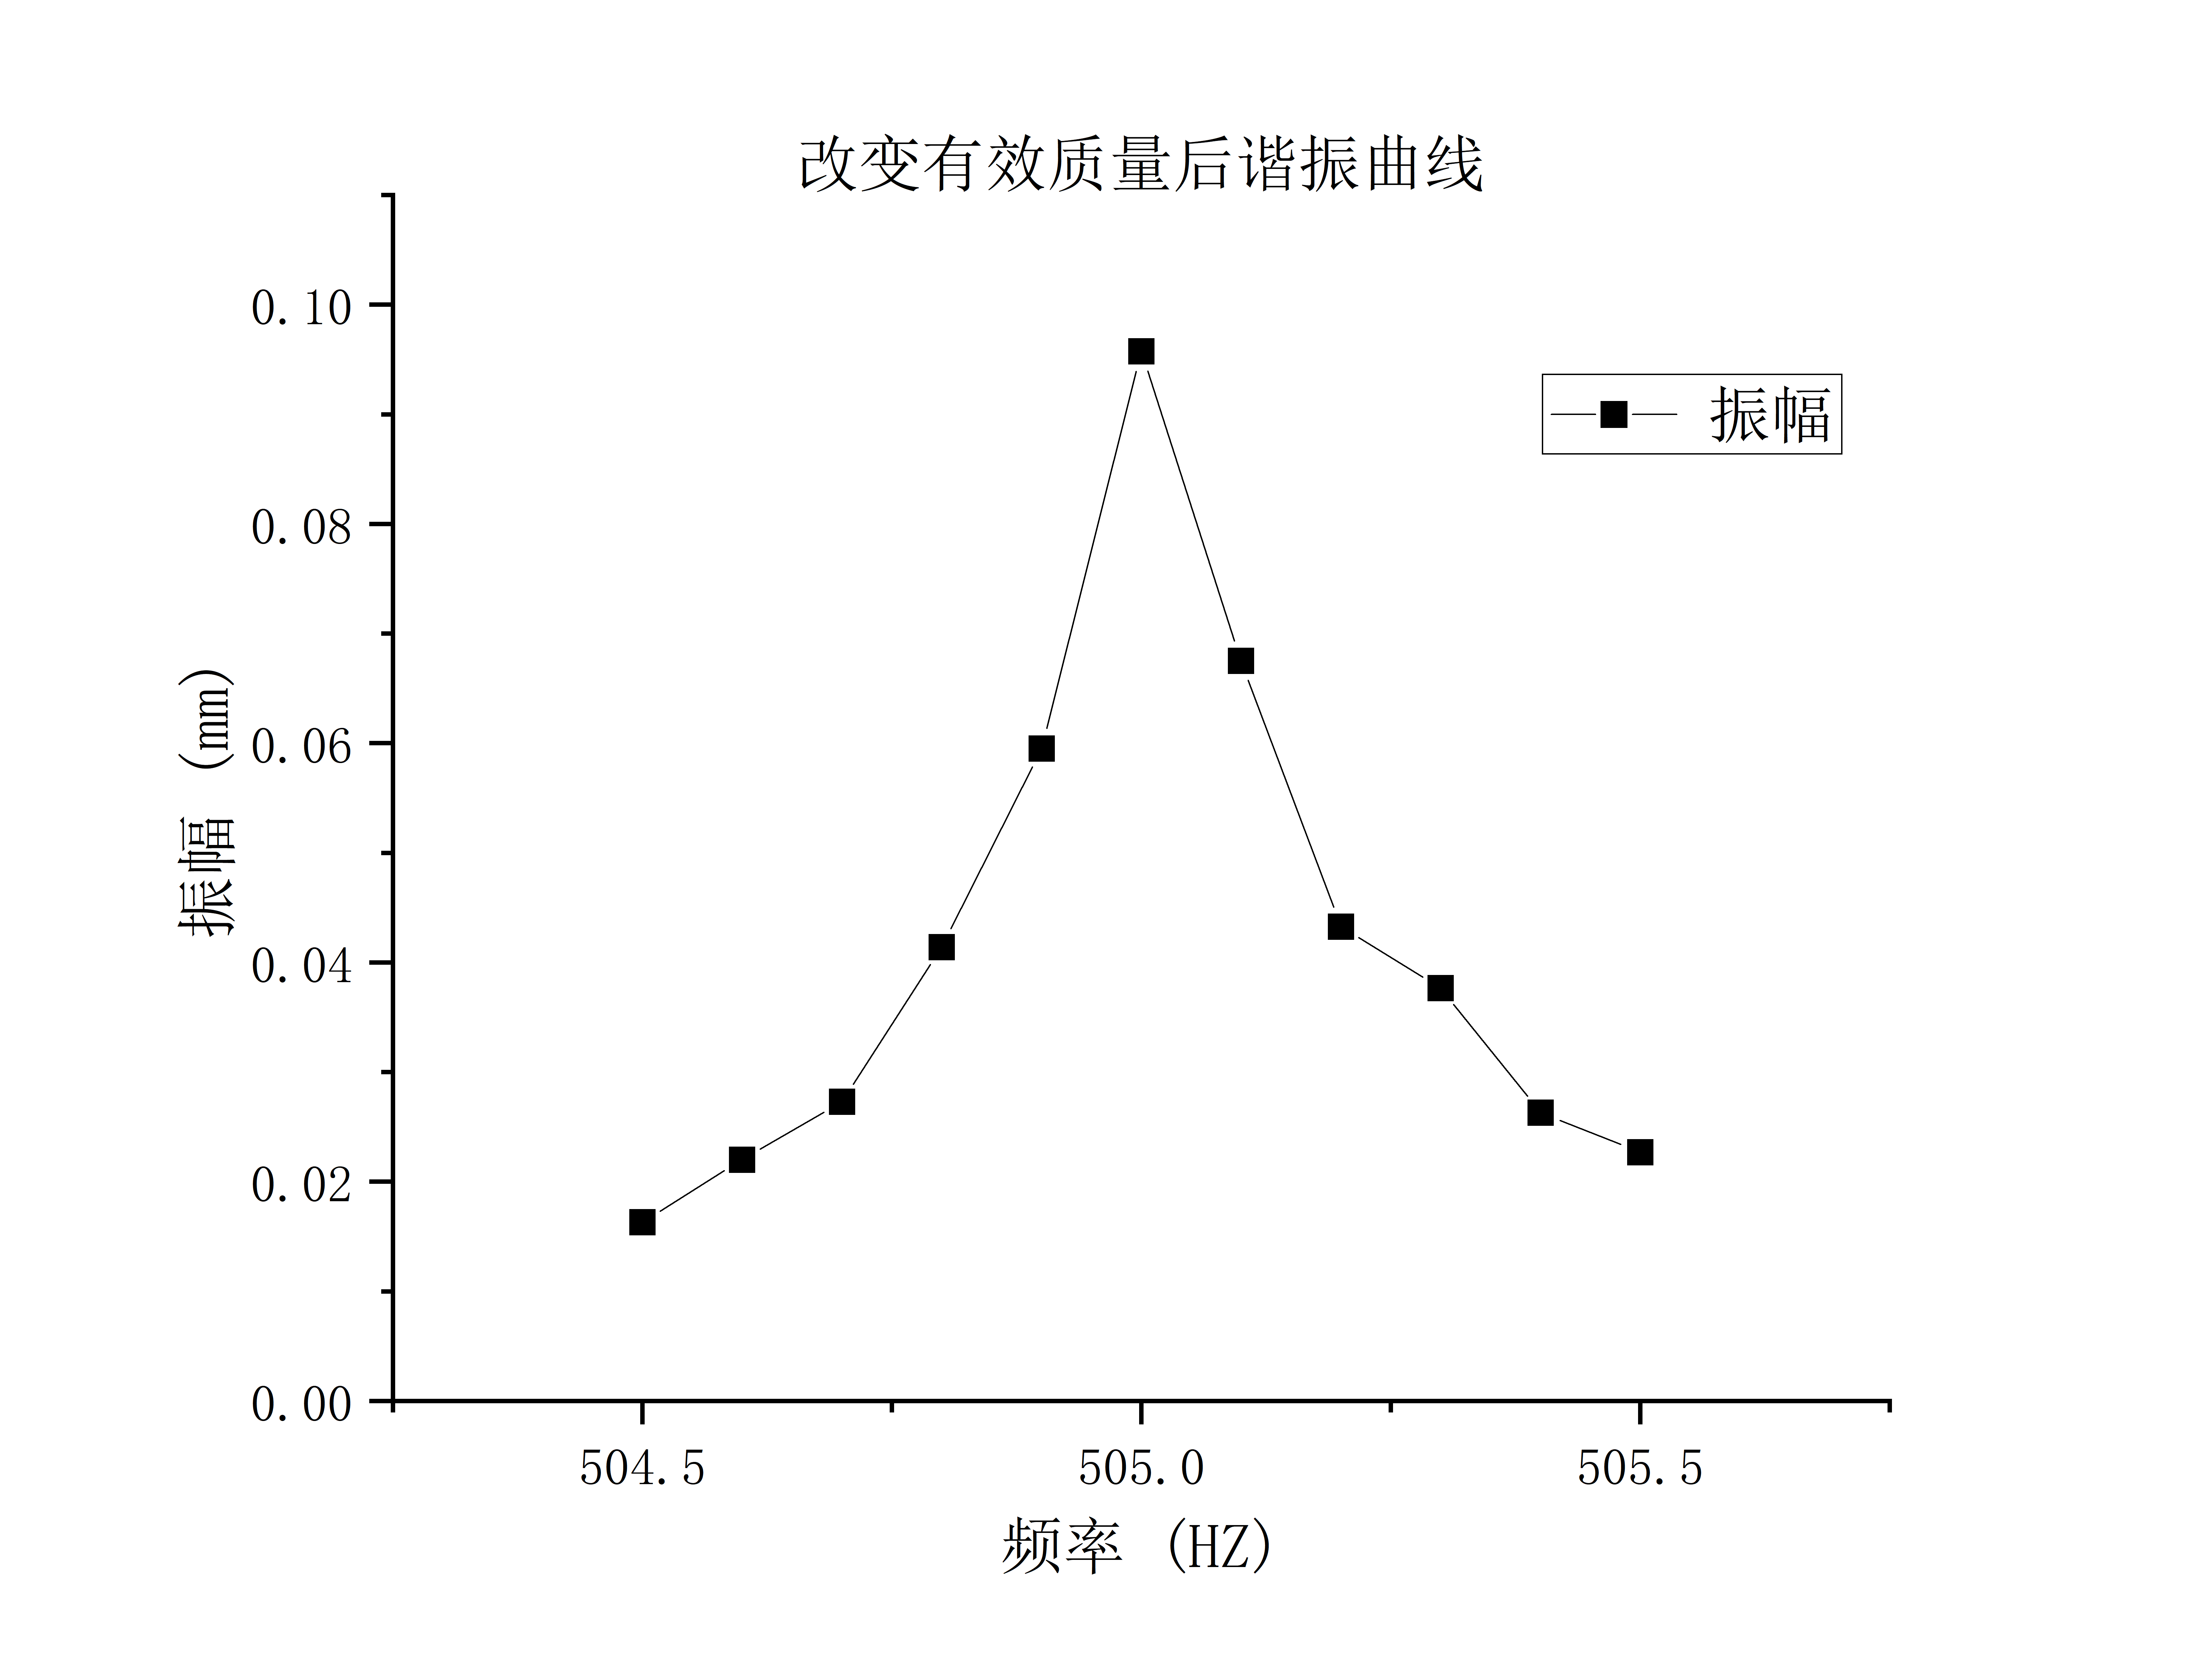
\includegraphics[width=0.8\linewidth]{images/改变有效质量}
		\caption{改变音叉的有效质量}
		\label{}
	\end{figure}
	% 结语部分
	\clearpage
	
	% 小标题
	\section{双光栅测量微弱振动位移量实验  \quad\heiti  后记}
	% ---
	
	% 总结、杂谈与致谢
	\subsection{实验心得和体会}
	\begin{enumerate}
		\item 这个实验的原理相对比较简单,类似迈克尔逊白光干涉实验,都是属于需要很大的耐心来调整光路,从而完成实验的,也感谢周老师和助教老师的帮助,让我很快完成了实验。
		\item 建议将改变有效质量的实验进一步深化,例如通过将软管放入不同位置的孔洞中,从而得到多组数据,更加直观有效的对 $\omega=\sqrt{\frac{k}{m}}$与谐振频率的关系有深刻的认识。
	\end{enumerate}
	% ---
	
	
	% ---
	
	% 附件
	\subsection{附件}
	\begin{figure}[H]
		\centering
		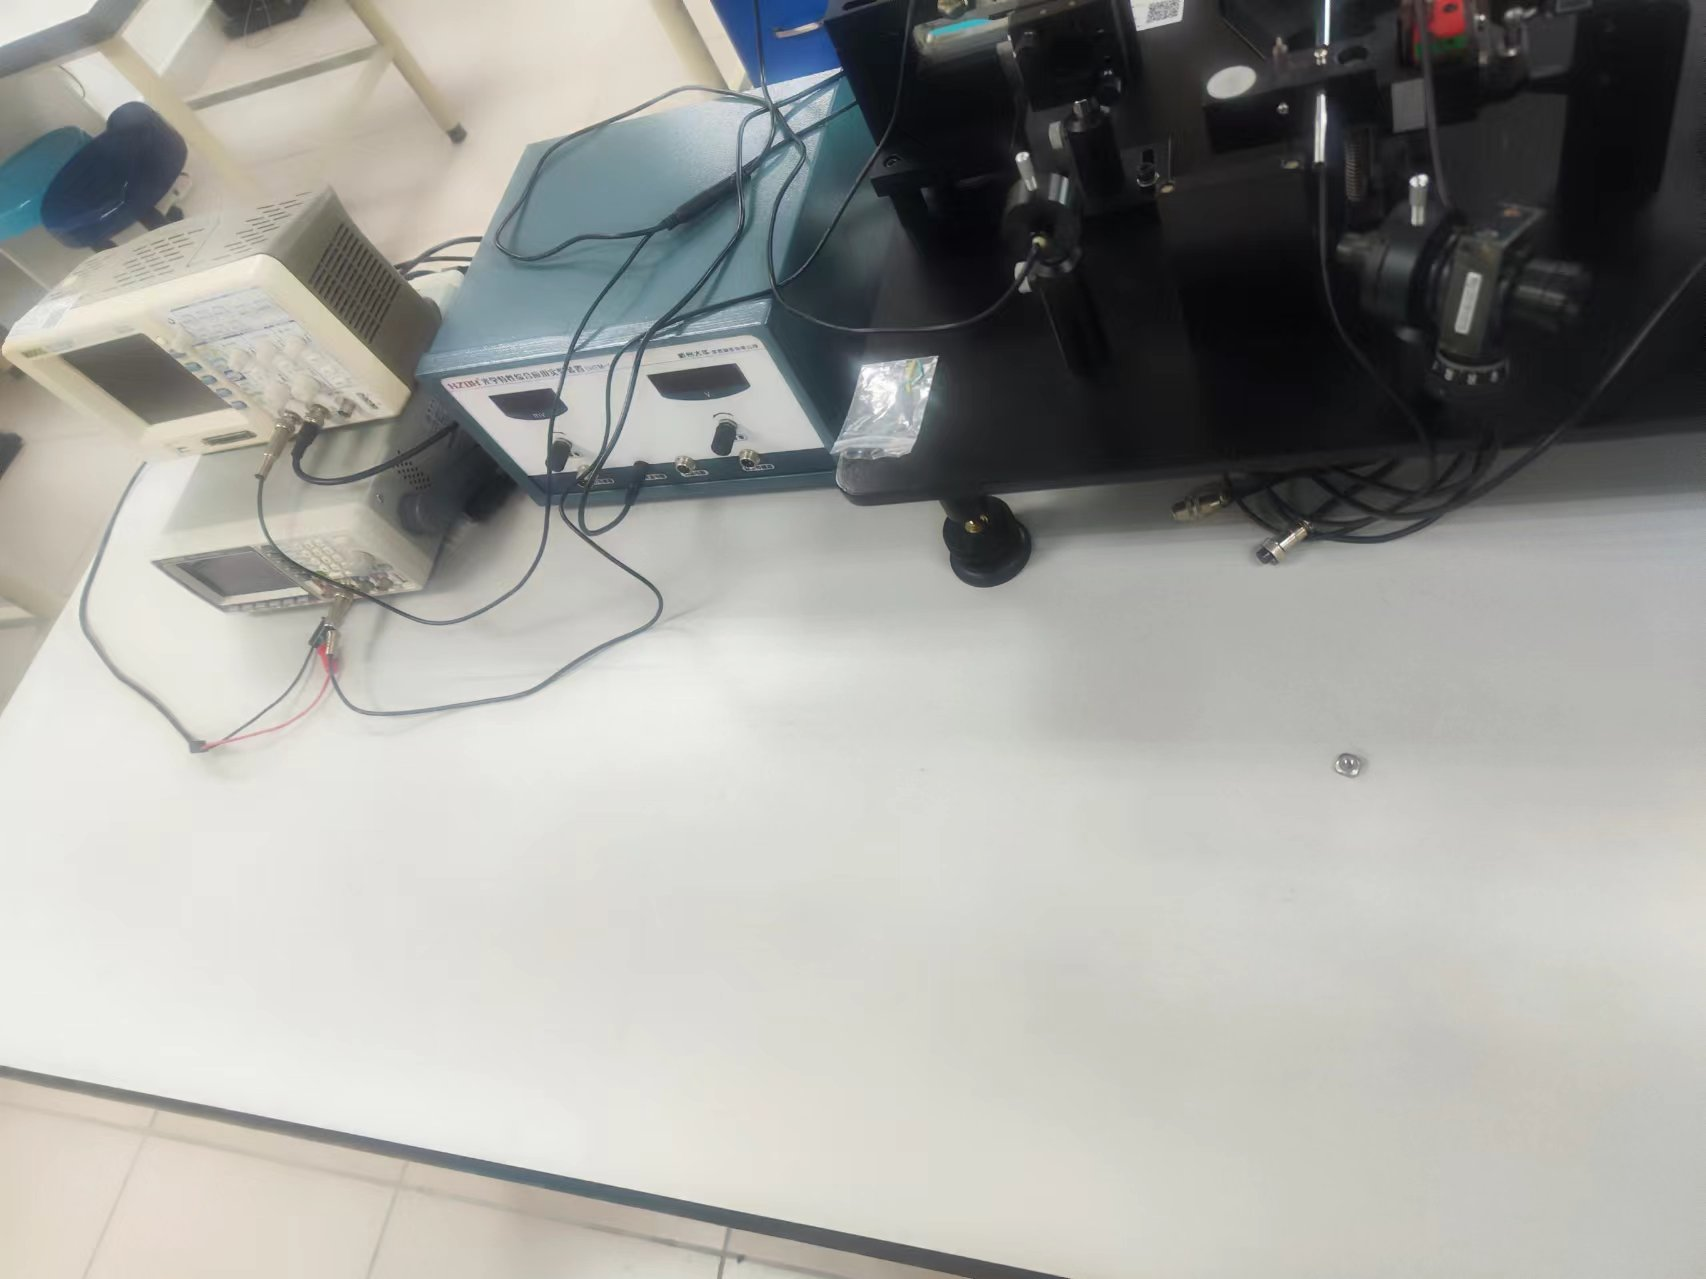
\includegraphics[width=0.4\linewidth]{images/桌面}
		\caption{实验桌面}
		\label{}
	\end{figure}
	\begin{figure}[H]
		\centering
		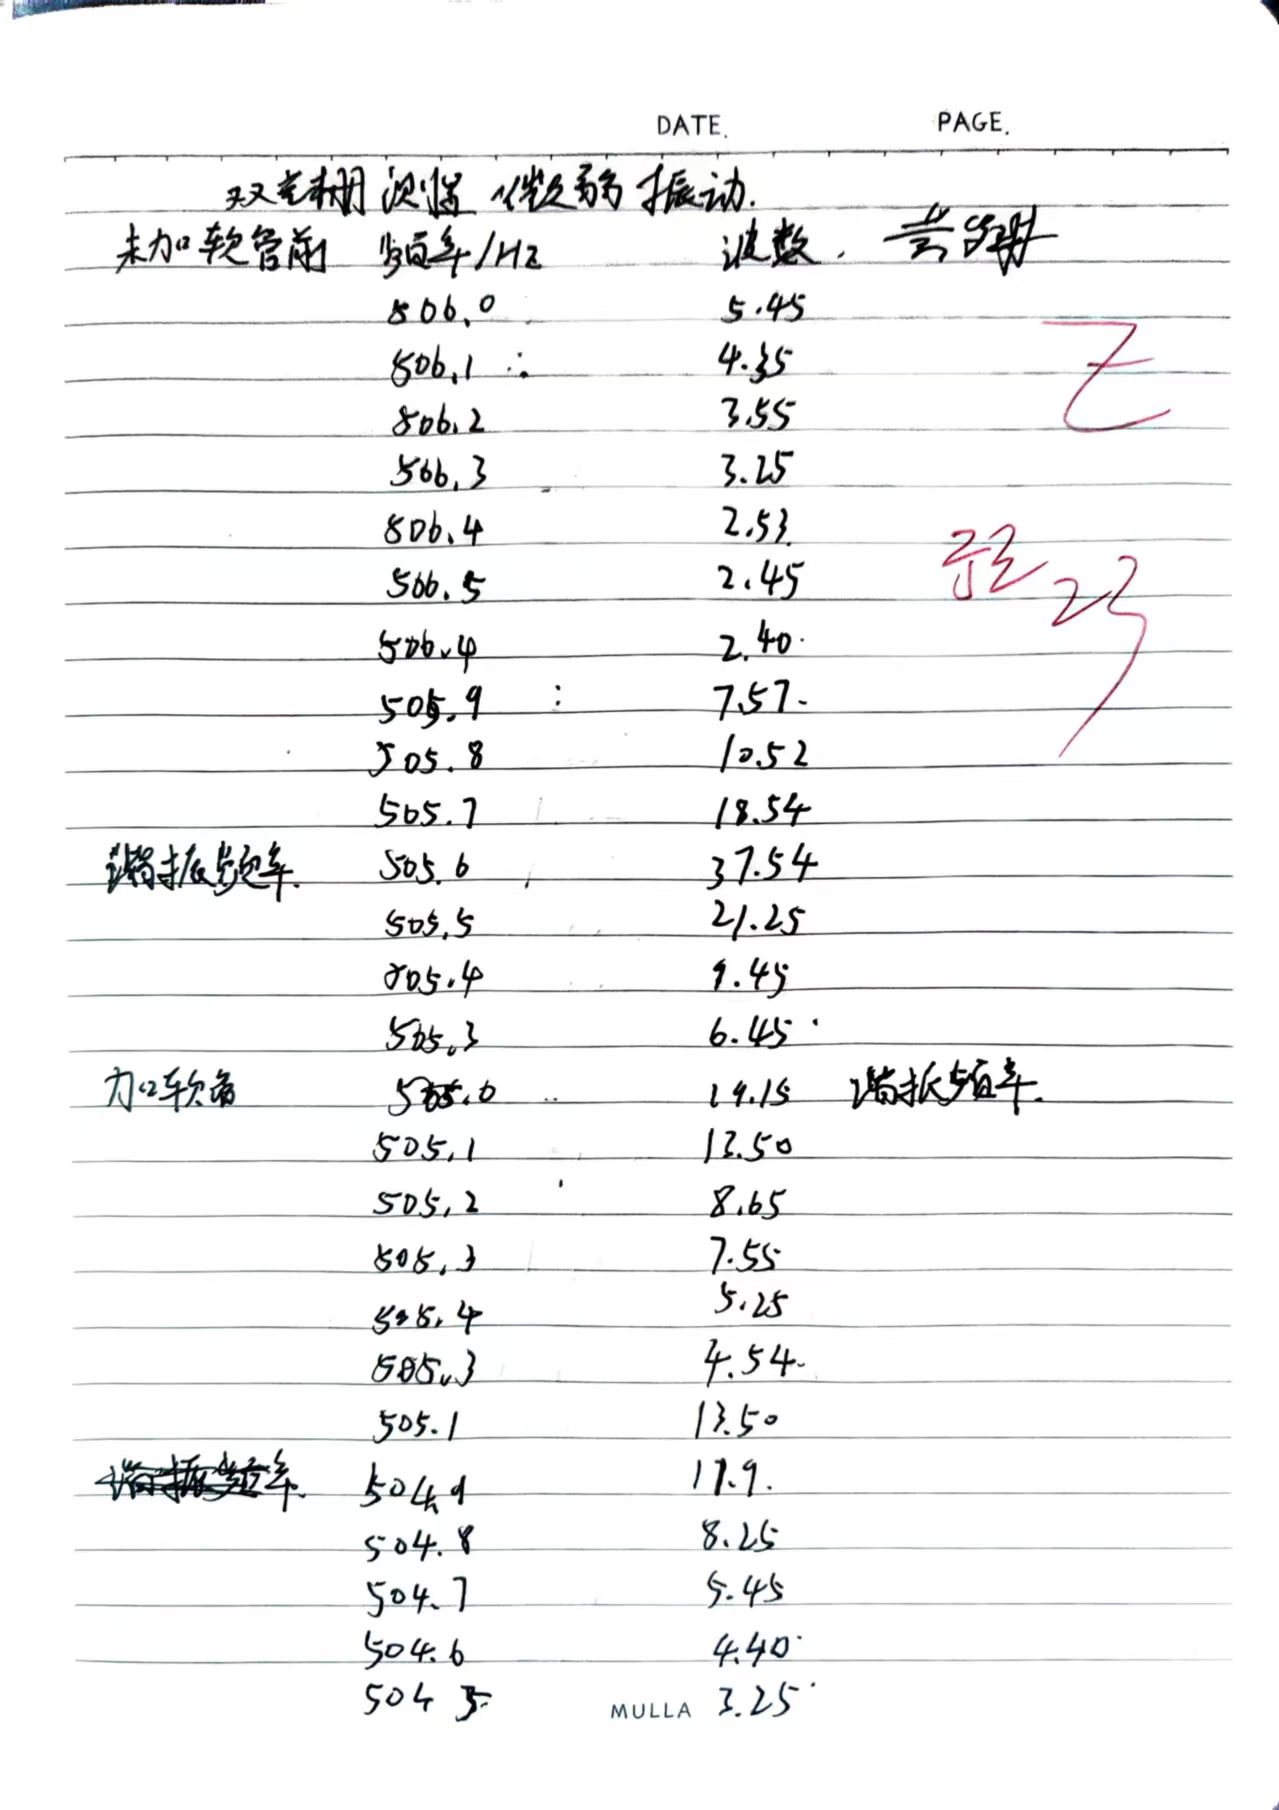
\includegraphics[width=0.3\linewidth]{images/原始数据}
		\caption{原始数据}
		\label{}
	\end{figure}
	
	
\end{document}